\chapter{Conceitos Básicos}
\label{sec:conceitos}

\section{Arquitetura de um jogo eletrônico multijogador com servidor central}
\label{sec:conceitos:servidores}
  Para quesito de comparação, é razoável termos em mente como se estrutura um jogo usual.
    
  \subsection{Separação do código}
    Um software cuja arquitetura de redes inclui um servidor central possui uma separação
    clara e bem definida de como um \textit{cliente} e um \textit{servidor} devem agir.
    
    \subsubsection{Software cliente}
      O software cliente é a parte que irá ser executada pelo público alvo do jogo, e é o que
      pode ser considerado como o "jogo em si". As escolhas de qual linguagem e/ou quais arcabouços
      utilizar, quais sistemas operacionais ou plataformas contemplar são todas realizadas em
      função do público alvo.
      Como jogos são interativos, essa parte sempre tem uma exigência de um ambiente gráfico,
      assim como uma placa de vídeo.
      
    \subsubsection{Software servidor}
      O software servidor é visado em um público mais técnico, podendo até mesmo ser restrito dentro
      da empresa. O objetivo principal do servidor é permitir que diversos clientes consigam manter
      suas simulações do mundo do jogo em sincronia. Para tal, a sincronização pode ser desde
      apenas sincronizar entrada, como até mesmo ser o único responsável pela simulação, tornando
      os clientes em apenas terminais burros.
      Em contraste com os clientes, as escolhas de linguagem, arcabouços, plataformas e outros são
      puramente econômicas, e não dependem das escolhas feitas para os clientes.
      
  \subsection{Integração}
    Tendo as duas partes separadas, elas não precisam ficar inteiramente separadas.
    
  \subsection{Comunidade}
    Uma forma que algumas empresas de colaborar com a comunidade de um jogo é de além de
    distribuir o cliente do jogo, distribuir um software para realizar exclusivamente a parte
    do servidor. Com acesso a esse software, chamado de \textit{servidor dedicado}, a comunidade
    pode por si só criar a manter servidores, que podem ser melhores que os oficiais para casos
    específicos

\section{Redes Peer-to-peer}
\label{sec:conceitos:redes}

  \begin{figure}[h]
    \begin{centering}
    \fbox{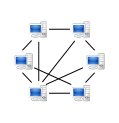
\includegraphics[width=0.45\textwidth]{../poster/p2p-network.png}}
    \fbox{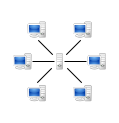
\includegraphics[width=0.45\textwidth]{../poster/server-based-network.png}}
    \caption{Comparação de rede Peer-to-peer (Esquerda) com Cliente-Servidor (Direita). \\
      Fonte: Baseado em figura de Wikimedia Commons}
    \end{centering}
  \end{figure}

  Uma rede peer-to-peer é um tipo de arquitetura de rede descentralizada e distribuída
  onde cada nó individual da rede atuam como consumidores e fornecedores de recursos,
  simultaneamente, em contraste com redes cliente-servidor onde nós clientes apenas
  requisitam serviços fornecidos por servidores centrais. \cite{peertopeer:definition}

\section{Vikings}
\label{sec:conceitos:vikings}
  O \textit{vikings}\footnotemark{} é um software livre produzido numa experiência de mini-projetos realizada pelo USPGameDev\footnotemark. 
  Foi desenvolvido em Janeiro e Fevereiro de 2013 por Henrique Gemignani Passos Lima e Wilson Kazuo Mizutani 
  utilizando a LÖVE, um arcabouço para jogos 2D em Lua\footnotemark{}.
  
  \begin{figure}
    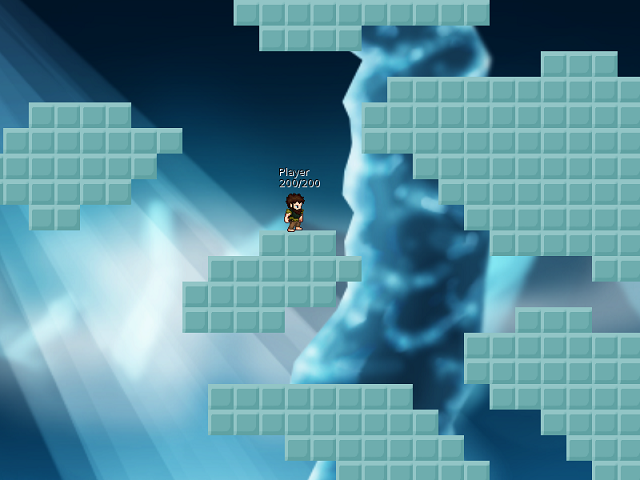
\includegraphics{imagens/vikings-1.png}
    \caption{Imagem do vikings}
  \end{figure}
  
  \addtocounter{footnote}{-3}

  \stepcounter{footnote}\footnotetext{
    Página do projeto: \url{http://uspgamedev.org/projetos/vikings/} (última visita em 23/11/2013).
  }
  \stepcounter{footnote}\footnotetext{
    O USPGameDev é um grupo de pesquisa e desenvolvimento de jogos da
    Universidade de São Paulo. Ver \url{http://uspgamedev.org/} (última visita em 03/09/2013).
  }
  \stepcounter{footnote}\footnotetext{
    Página oficial: \url{http://www.lua.org/} (última visita em 23/11/2013).
  }

  \subsection{O Jogo}
    Em \textit{vikings}, você controla um jovem viking que sonha em se tornar o líder de sua vila. Para tal,
    você sai em busca de aventuras, buscando experiência, riquezas e equipamentos poderosos, para que um dia,
    você seja forte o suficiente para desafiar e derrotar o seu líder, tomando o seu lugar.
        
  \subsection{Jogabilidade}
    É um jogo de plataforma 2D com gráficos 2D, com mapas gerados procedimentalmente. Com o intuito de garantir
    que todo mapa gerado é possível, e numa tentativa de introduzir alguma profundidade e dificuldade, é
    possível dar quantas \textit{arrancadas} você quiser, mesmo estando no ar, e um único pulo no ar. No
    entanto, bater com a sua arma numa parede concede mais um pulo, permitindo ao jogador que ele escale
    paredes.
    
  \subsection{Detalhes Técnicos}
    Uma lista de conceitos e/ou algorítimos interessantes presentes no código:
    
    \subsubsection{Orientação a Objetos}
      Lua não possui orientação a objetos nativamente, mas utilizando as ferramentas da linguagem é possível
      implementar um sistema de orientação a objetos baseada em protótipos.
      No projeto, utilizamos o LUX\footnotemark{}, escrito pelo próprio Wilson, em vez de repetir uma implementação.
      
      \footnotetext{
        Página do projeto: \url{https://github.com/Kazuo256/luxproject} (última visita em 23/11/2013).
      }
    
    \subsubsection{Geração procedimental de conteúdo}
      Para a geração dos mapas de cavernas, utilizamos o algorítimo de automato celular, descrito no RogueBasin,
      \cite{roguebasin:cellularautomata} e levemente alterado para criar plataformas mais largas. Para
      evitar problemas de áreas desconexas, há um tratamento posterior do mapa onde áreas desconexas são unidas.
      Por fim, procuramos por plataformas vazias onde popular com monstros e itens.